\documentclass{beamer}
\usetheme{Warsaw}
\usetheme{CambridgeUS}
\usefonttheme{structuresmallcapsserif}
\usefonttheme{serif}
\useinnertheme{circles}

\setbeamertemplate{background canvas}[vertical shading][bottom=white,top=white]   
\setbeamercolor{math text}{fg=black!10!Lublue}
\setbeamercolor{block title}{bg=blue!40!white, fg=black}
%\setbeamertemplate{navigation symbols}{}
\setbeamerfont{frametitle}{size=\normalsize}

\definecolor{light-gray}{gray}{0.99}
\definecolor{light-blue}{rgb}{0.90,0.90,0.98}
\definecolor{light-yellow}{rgb}{0.95,0.95,0.10}
\definecolor{dark-green}{rgb}{0.10,0.50,0.10}
\definecolor{Lublue}{rgb}{.10,.10,.70}
\definecolor{links}{rgb}{0.05,0.05,0.95}
\hypersetup{colorlinks,linkcolor=,urlcolor=links}

\definecolor{UNAMoro}{rgb}{0.796, 0.671, 0.341} % (secondary)
\definecolor{UNAMblue}{rgb}{0.067, 0.129, 0.275} % (primary)

%\setbeamercolor{palette primary}{bg=UNAMblue,fg=white}
%\setbeamercolor{palette secondary}{bg=UNAMblue,fg=white}
\setbeamercolor{palette tertiary}{bg=UNAMblue,fg=white}
%\setbeamercolor{palette quaternary}{bg=UNAMblue,fg=white}
\setbeamercolor{structure}{fg=UNAMblue} % itemize, enumerate, etc
\setbeamercolor{section in toc}{fg=UNAMblue} % TOC sections
\setbeamercolor{subsection in toc}{fg=Lublue} % TOC sections
% Override palette coloring with secondary
\setbeamercolor{subsection in head/foot}{bg=UNAMoro,fg=UNAMblue}
\setbeamercolor{frametitle}{bg=UNAMoro,fg=UNAMblue}
\setbeamercolor{subtitle}{bg=UNAMoro,fg=UNAMblue}

\usepackage[utf8]{inputenc}
\usepackage[spanish]{babel}
\usepackage{amsmath}
\usepackage{amsfonts}
\usepackage{amssymb}
\usepackage{empheq}
\usepackage{graphicx}
\usepackage{color}
\usepackage{listings}
\usepackage{hyperref}
\usepackage{wasysym}
\usepackage{alltt}
\usepackage{algorithmic}
\usepackage{cancel}
\usepackage[export]{adjustbox}
\usepackage{caption}
\usepackage{tikz}
\usetikzlibrary{arrows,backgrounds}
\tikzstyle{block}=[draw opacity=0.7,line width=1.4cm]

\graphicspath{{./Figuras/}{../Figuras/}}


%%%%%%%%%%%%%%%%%%%%%%%%%%%%%% User specified LaTeX commands.
\newcommand{\Vector}[1]{{\mathbf{#1}}}
\newcommand{\Tensor}[1]{\underline{\underline{\mathbf{#1}}}}
\newcommand*\widefbox[1]{\fbox{\hspace{1em}#1\hspace{1em}}}
%%%%%%%%%%%%%%%%%%%%%%%%%%%%%%
% Definimos el punto decimal.
\spanishdecimal{.}
%%%%%%%%%%%%%%%%%%%%%%%%%%%%%%

% the beginning of each subsection:
\AtBeginSection[]
{
	\begin{frame}<beamer>{Contenido}
		\tableofcontents[currentsection]
	\end{frame}
}

\title[PAPIME--PE101019]{Diferencias Finitas}   
\subtitle{Problemas estacionarios I}

\author[\copyright LMCS]{ \textcolor{UNAMblue}{Modelación computacional en las ciencias y las ingenierías como apoyo en el proceso enseñanza-aprendizaje\\(PAPIME-PE101019)}} 
\institute[IGEF--UNAM] 
{ 
	{\small{Instituto de Geof\'isica}} \\ 
	\vspace{0.15cm}
	{\small{Universidad Nacional Aut\'onoma de M\'exico}} \\
	\vspace{0.15cm}
	
\includegraphics[height=.85cm]{unamlogo.png} 
}

\date[2019--2021]{\\ {\tiny{Esta obra está bajo una 
			\href{https://creativecommons.org/licenses/by-nc-sa/4.0/}{Licencia Creative Commons Atribución-NoComercial-CompartirIgual 4.0 Internacional.}}\\
		
\includegraphics[scale=0.20]{ccPyNoxtli.png}}}

% To uncover everything in a step-wise fashion:
%\beamerdefaultoverlayspecification{<+->}

\begin{document}
	
\begin{frame}
\titlepage
\end{frame}

\begin{frame}{Contenido}
\tableofcontents
\end{frame}

\section{Conducción de calor}

\subsection{Modelo Conceptual}

\begin{frame}{}

{\huge MODELO}
$$
\includegraphics[height=1.5cm]{conceptualCOMPLETO}$$

\end{frame}

\begin{frame}{¿Qué es la transferencia de calor? \cite{Bergman}}

Cuando estudiamos termodinámica, aprendemos que la energía se puede transferir mediante 
interacciones de un sistema con el ambiente que lo rodea.

\strut

Estas interacciones se llaman \textit{trabajo} y \textit{calor}.

\strut

Sin embargo, en termodinámica se estudian los estados finales de los procesos, durante los
que ocurren las interacciones, pero no se provee información de la naturaleza de las 
interacciones o de la velocidad a la que ocurren.

\end{frame}

\begin{frame}{¿Qué es la transferencia de calor? \cite{Bergman}}

\textbf{Calor}: forma de la energía que se puede transferir de un sistema a otro como resultado
de la diferencia en la temperatura.

\textbf{Transferencia de calor}: determinación de las razones de esa transferencia de energía.

\begin{columns}
	\begin{column}{0.5\textwidth}
$$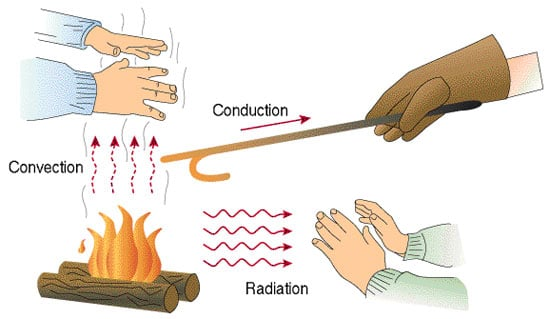
\includegraphics[width=6cm]{TransDeCalor.jpg}$$
	\end{column}
	\begin{column}{0.5\textwidth}
\begin{description}
	\item[Conducción] gradiente de temperaturas en un medio estacionario.
	\item[Convección] ocurre entre una superficie y un fluido en movimiento cuando están a diferentes temperaturas.
	\item[Radiación] calor emitido en forma de ondas electromagnéticas.
\end{description}
	\end{column}
\end{columns}

\end{frame}


\begin{frame}
\begin{center}
	\fcolorbox{light-gray}{light-gray}{{\Huge \textcolor{black}{Conducción de calor}}}
\end{center}
\end{frame}

\begin{frame}{Conducción de calor \cite{Bergman}}

{\small 
Es posible cuantificar los procesos de transferencia de calor en términos de \textit{ecuaciones de cambio},
que se pueden usar para calcular la cantidad de energía transferida por unidad de tiempo.

\strut

Dada una distribución de temperaturas $T(x)$, la \textbf{Ley de Fourier} para la conducción de calor es:
%
\[
\boxed{q_x^{\prime\prime} = -\kappa \frac{d T}{d x}}
\]

\strut

$q_x^{\prime\prime}$ (W/m$^2$) representa la velocidad con que se transfiere el calor en dirección $x$ por unidad de área perpendicular a la dirección
de transferencia. También se conoce como \textit{flujo de calor} o \textit{transferencia de calor por unidad de área}.

\strut
		
$\kappa$ (W/m$\cdot$K) es una propiedad del material que representa a la \textbf{conductividad térmica}.
}

\end{frame}

\begin{frame}{Conducción de calor \cite{Bergman}}
	
\begin{columns}
	\begin{column}{0.25\textwidth}
	$$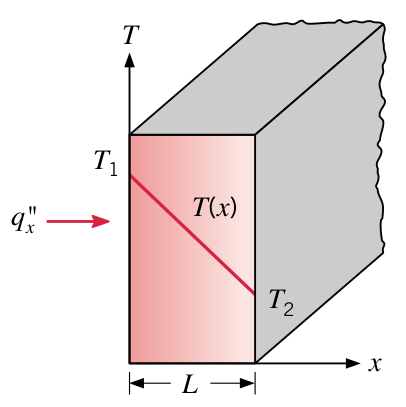
\includegraphics[scale=0.25]{Fourier.png}$$
	\end{column}
	\begin{column}{0.75\textwidth}	
	{\small
	En la figura observamos la representación de un material con temperatura $T_1$ en una cara y $T_2$ en la otra.
	En este caso, se considera un estado estacionario (no depende del tiempo) y que la transferencia de calor es en una dimensión
	y en dirección $x$. Observamos que en este caso la $T(x)$ es una función lineal.
    }
	\end{column}
\end{columns}

{\small 
Entonces el gradiente de temperaturas se puede escribir como $\displaystyle d T / d x = (T_2 - T_1) / L$,
por lo tanto, el flujo de calor sería:
\[  q_x^{\prime\prime} = -\kappa \frac{T_2 - T_1}{L} = \kappa \frac{\Delta T}{L}\]
%
donde $\Delta T = T_1 - T_2$.
Finalmente, la \textbf{transferencia de calor por conducción} $q_x$ (W), 
a través de una pared plana de área $A$, es: $q_x = q_x^{\prime\prime} \cdot A$ .
}

\end{frame}

\begin{frame}

\begin{block}{Ejemplo: Horno industrial \cite{Bergman}}
{\footnotesize La pared de un horno industrial está construida de ladrillos de arcilla refractaria
cuya conductividad térmica es de $1.7$ W/m$\cdot$K. En estado estacionario, durante su
operación, la temperatura interna tiene una temperatura de 1400 K, mientras que la
externa 1150 K. Si la pared es de $0.5$ m $\times$ $1.2$ m, ¿cuál es la razón de pérdida
de calor ($q_x$) a través de la pared?}
$$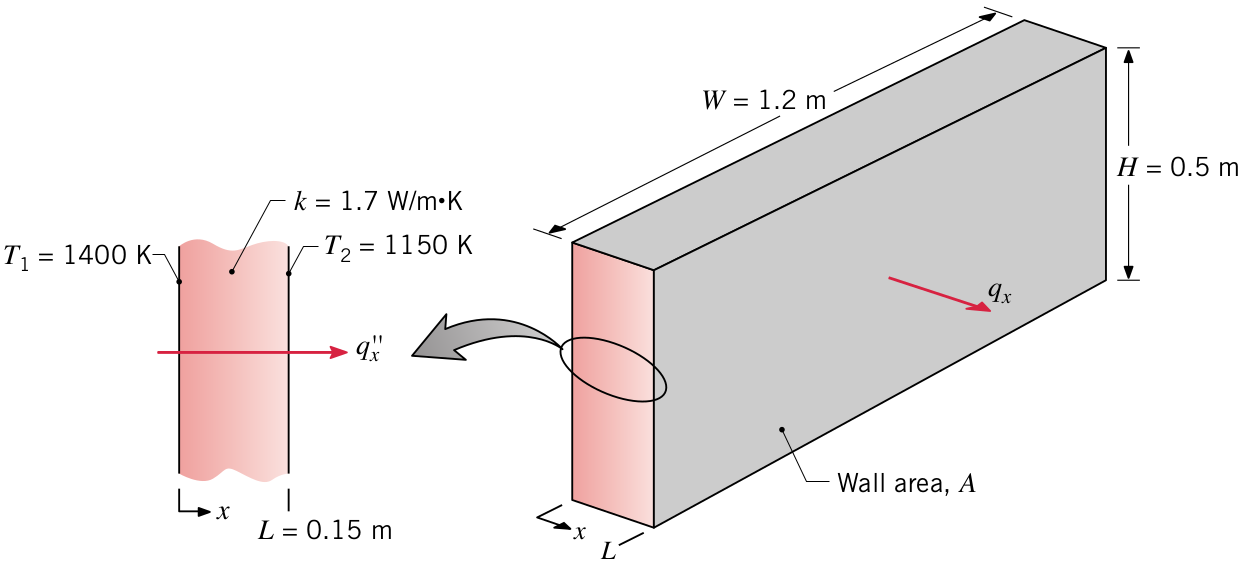
\includegraphics[scale=0.35]{EjemploConduccion1D.png}$$
\end{block}
\end{frame}

\begin{frame}

\begin{block}{Ejemplo: Horno industrial \cite{Bergman}}
Tomando en cuenta la dirección del flujo de calor, es posible calcular $q_x^{\prime\prime}$ usando la Ley de Fourier:
\[
q_x^{\prime\prime} = \kappa \frac{\Delta T}{L} = 1.7 \text{W/m}\cdot\text{K} \times \frac{1400\text{K} - 1150\text{K}}{0.15 \text{m}} = 2833 \text{W/m}^2
\]

Para conocer la pérdida de calor a través de la pared (transferencia de calor por conducción) multiplicamos $q_x^{\prime\prime}$ por el área de la pared:
\[
q_x = q_x^{\prime\prime} \cdot A = 2833 \text{W/m}^2 \times (0.5 \text{m} \times 1.2 \text{m}) = \boxed{1700 \text{W}} .
\]


\end{block}
\end{frame}

\begin{frame}

Supongamos ahora, que deseamos conocer la distribución de temperaturas al interior de la pared del horno.

$$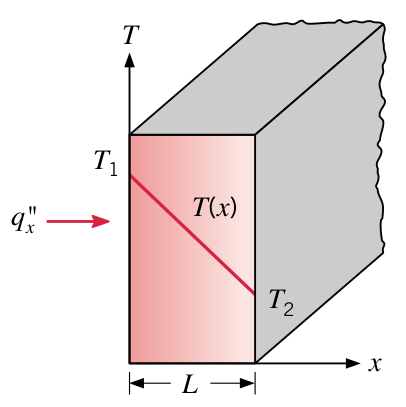
\includegraphics[scale=0.25]{Fourier.png}$$
	
Para ello debemos plantear varias hipótesis y obtener un modelo matemático para $T(x)$.

\strut

La solución de ese modelo matemático, analítica y/o numérica, darán la distribución de temperaturas buscada. 
\end{frame}


\begin{frame}{Conducción de calor en 1D}

Para fijar ideas, vamos a estudiar la transferencia de calor en un dominio como el que se muestra en la siguiente figura:
$$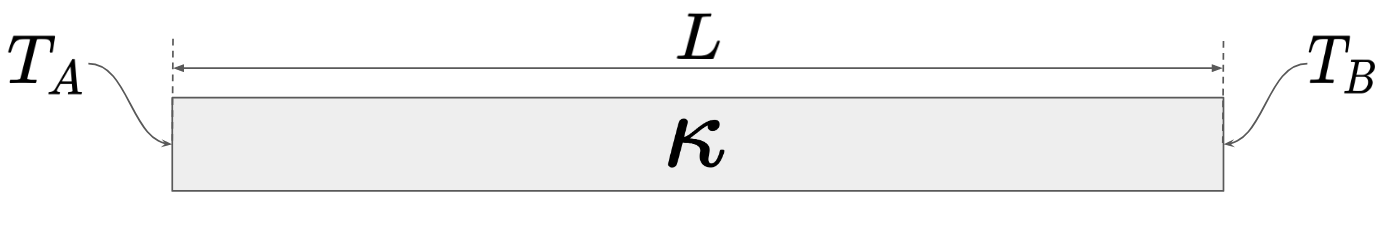
\includegraphics[scale=0.30]{ModCon01.png}$$

{\small 
\begin{itemize}
	\item Consideramos que no hay de flujo de calor en las paredes horizontales (son adiabáticas).
	\item Tenemos temperaturas $T_A$ y $T_B$ fijas en los extremos.
	\item No se consideran fuentes ni sumideros.
    \item $\kappa$ representa la conductividad térmica.
    \item En este problema se desea calcular la temperatura $T$ al interior del dominio.
    \item Como primera aproximación, el dominio se considera unidimensional.
\end{itemize}
}

\end{frame}

\subsection{Modelo Matemático}

\begin{frame}{}

{\huge MODELO}
$$
\includegraphics[height=1.5cm]{matematicoCOMPLETO}$$

\end{frame}

\begin{frame}

{\footnotesize 
Ecuación ``general'' de transferencia de calor (véase \cite{Herrera1}):
%
\begin{equation*}
\boxed{
c_p \rho \frac{\partial T}{\partial t} +
c_p \rho \frac{\partial}{\partial x_j} \left( u_j T \right) -
\frac{\partial }{\partial x_j} \left( \kappa \frac{\partial T}{\partial x_j}\right) = 
S} \qquad \text{(índices repetidos se suman)}
\end{equation*}
%
donde se define lo siguiente:
%
}
{\footnotesize 
\begin{center}
\begin{tabular}[h!]{cp{8cm}c}
	\textbf{Símbolo} &  & \textbf{Unidades} \\
	\hline
	\multicolumn{3}{c}{\textbf{Parámetros físicos}}\\
	$c_p$    & Capacidad calorífica específica. & [J / Kg $^\text{o}$K]\\
	$\rho$    & Densidad. & [Kg / m$^3$]\\
	$\kappa$ & Conductividad térmica. &  [W / m $^\text{o}$K] \\
	$S$ & Ganancia (fuente) o pérdida (sumidero) de calor & [J/m$^3$ s] \\
	
	$\displaystyle \alpha = \frac{\kappa}{c_p \rho}$ & Difusividad térmica. & [m$^2$/s] \\ \\
	\hline
	\multicolumn{3}{c}{\textbf{Variables independientes}}\\
	$x_j$    & Coordenadas cartesianas: $(x_1, x_2, x_3) \equiv (x, y, z)$. & [m] \\
	$t$      & Tiempo. & [s] \\
	\hline
	\multicolumn{3}{c}{\textbf{Variables dependientes}}\\
	$T$    & Temperatura. & [$^\text{o}$K] \\
	$u_j$ & Componentes de la velocidad: $(u_1, u_2, u_3) \equiv (u_x, u_y, u_z)$. & [m/s] \\
	\hline
\end{tabular}
\end{center}
}

\end{frame}

\begin{frame}
	
{\small 
Dado que estamos interesados en la conducción de calor estacionaria eliminamos el
término temporal y el término de advección de la ecuación general:
%
\begin{equation*}
\cancelto{}{c_p \rho \frac{\partial T}{\partial t}} +
\cancelto{}{c_p \rho \frac{\partial}{\partial x_j} \left( u_j T \right)} -
\frac{\partial }{\partial x_j} \left( \kappa \frac{\partial T}{\partial x_j}\right) = 
S
\end{equation*}
%
Entonces, el modelo matemático para este problema en 1D y con $\kappa = constante$ es:
%
\begin{empheq}[box=\widefbox]{align}
-\kappa \frac{d^2 T}{d x^2} & = S \label{eq:conduccion1D} \\
T(x = 0) & = T_A \nonumber \\
T(x = L) & =  T_B \nonumber
\end{empheq}

Obsérvese que se tienen condiciones de tipo \textcolor{blue}{Dirichlet}: la variable dependiente, $T$, está dada en las fronteras.
Estas condiciones también se conocen como de \textcolor{blue}{primer tipo}.	
}

\end{frame}


\subsection{Modelo Numérico}

\begin{frame}

{\huge MODELO}
$$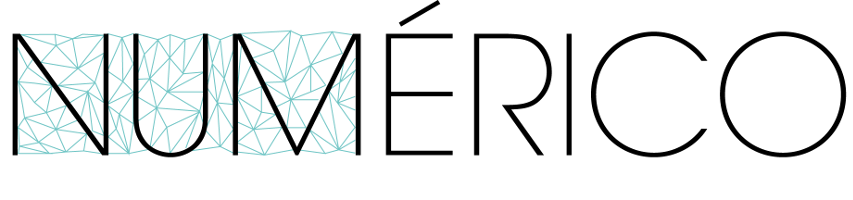
\includegraphics[height=1.75cm]{numericoCOMPLETO}$$

\end{frame}

\begin{frame}

\begin{description}
	\item[Discretización]  Proceso de transferir funciones continuas, modelos, variables y ecuaciones a sus contrapartes \textit{discretas}. 
\end{description}
\begin{itemize}
	\item {\small  La discretización es el primer paso en un modelo numérico cuyo objetivo es generar las contrapartes \textit{discretas} de manera adecuada, para que posteriormente sean evaluadas numéricamente mediante algoritmos que se implementan en una computadora.}
	
	\strut
	
	\item {\small La RAE define \textbf{Discreto}: 5. \textcolor{blue}{\textit{adj. Mat.}} Dicho de una magnitud: Que toma valores distintos y separados. 
		Por ejemplo: \textit{la sucesión de los números enteros es discreta, pero la temperatura no}.}
\end{itemize}
%
\end{frame}

\begin{frame}{Por ejemplo}
%
\begin{columns}
	\begin{column}{0.5\textwidth}
		{\small En la gráfica de la derecha, la línea azul representa una función continua,
			mientras que los puntos negros, conectados con una línea naranja, representan 
			una discretización que intenta aproximar a la función.}
		\vspace{0.25cm}
	\end{column}
	\begin{column}{0.5\textwidth}
		$$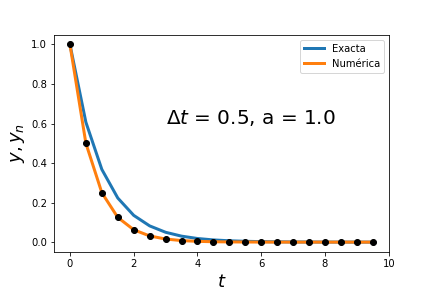
\includegraphics[scale=0.30]{Ejemplo03_1.png}$$
		\vspace{0.25cm}
	\end{column}
\end{columns}
%
\begin{columns}
	\begin{column}{0.60\textwidth}
		$$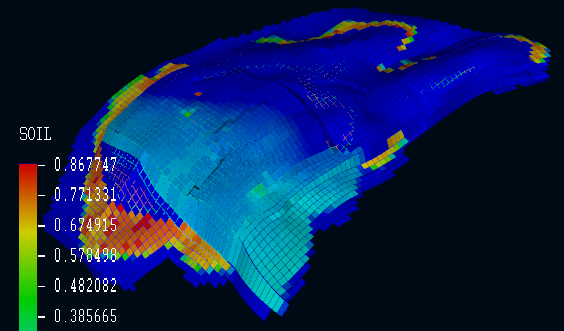
\includegraphics[scale=0.28]{MallaMay.png}$$
	\end{column}
	\begin{column}{0.40\textwidth}
		{\small En la figura de la izquierda, se observa la discretización de un yacimiento
			petrolero en varias celdas o elementos.}
		\vspace{1cm}
	\end{column}
\end{columns}

\end{frame}

\subsubsection{Discretización del dominio}

\begin{frame}
\begin{center}
	\fcolorbox{light-gray}{light-gray}{{\Huge \textcolor{black}{Discretización del dominio}}}
\end{center}
\end{frame}

\begin{frame}{Discretización del dominio}

El primer paso en nuestro modelo numérico es discretizar el dominio:

$$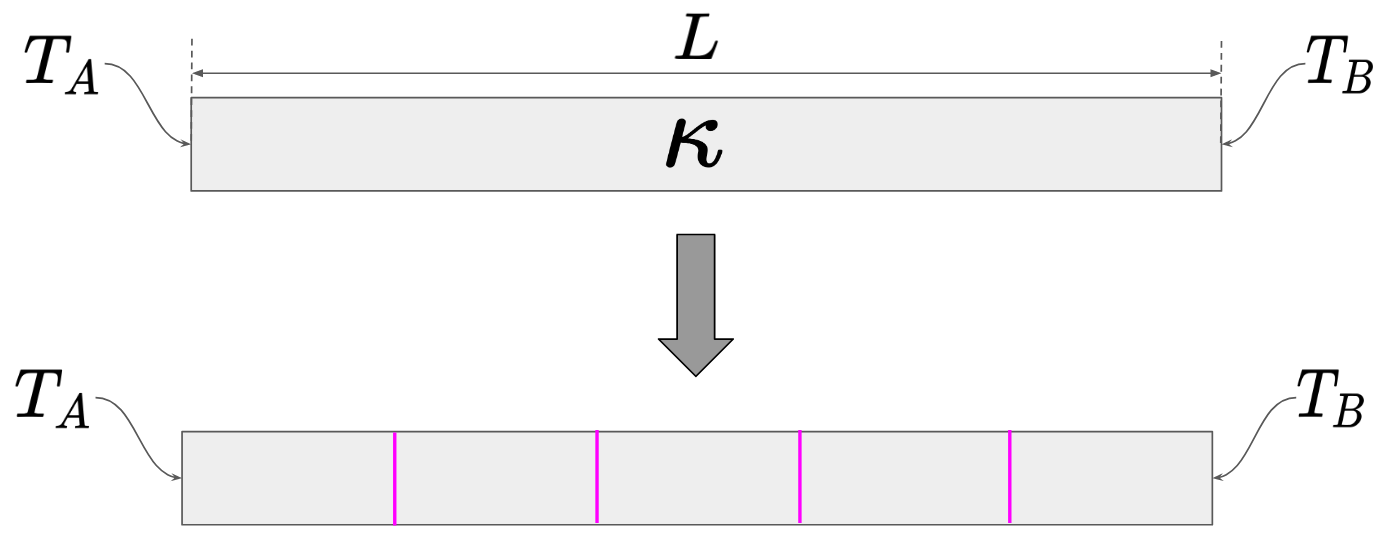
\includegraphics[scale=0.30]{ModCon02.png}$$

Como se observa en la figura, el dominio se ha partido en varios \textit{subdominios}.

\end{frame}

\begin{frame}{Discretización del dominio}

Una vez hecha la partición del dominio, es importante identificar los lugares del dominio
donde se va a calcular la temperatura. 
$$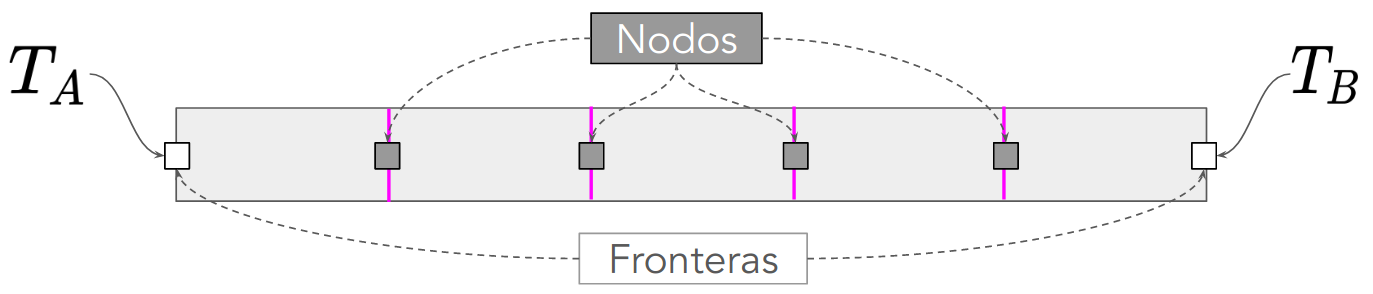
\includegraphics[scale=0.30]{ModCon03.png}$$
En la figura, se han identificado los \textit{nodos} en el interior del dominio (cuadros grises).
\begin{itemize} 
\item \textcolor{blue}{Es en estos nodos donde se hará el cálculo.}
\end{itemize}
También se identifican dos nodos especiales, los cuales están en los extremos del dominio (cuadros blancos).
\begin{itemize} 
\item \textcolor{blue}{En esos nodos se imponen las condiciones de frontera.}
\end{itemize}

\end{frame}

\begin{frame}{Discretización del dominio}

El siguiente paso es numerar los nodos:
$$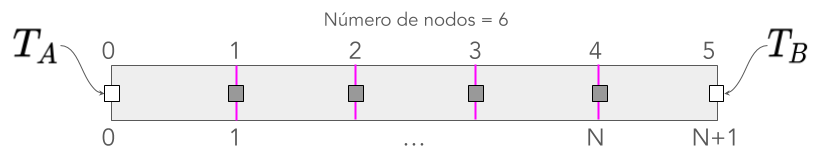
\includegraphics[scale=0.35]{ModCon04.png}$$

\textbf{Observaciones}:
	
{\small 
\begin{itemize}
\item La numeración la comenzamos en $0$.

\item Los nodos donde se va a calcular la temperatura $T$ van de $1$ a $N=4$.
Se dice que se tienen 4 grados de libertad, es decir, 4 incógnitas que se deben calcular.

\item Las fronteras están identificadas en: $i=0$ e $i= 5 (=N+1)$.

\item La discretización del domino genera lo que se conoce como \textcolor{blue}{\textit{malla del dominio}}, la cual
define las coordenadas de los nodos y en varios casos también conectividades.
\end{itemize}
}

\end{frame}

\subsubsection{Discretización de las ecuaciones}

\begin{frame}
\begin{center}
	\fcolorbox{light-gray}{light-gray}{{\Huge \textcolor{black}{Discretización de las ecuaciones}}}
\end{center}
\end{frame}

\begin{frame}{Discretización de las ecuaciones}
Recordemos que el modelo matemático consta de la siguiente ecuación:
\[
-\kappa \frac{d^2 T}{d x^2} = S
\]

Discretizamos la ecuación usando diferencias finitas de segundo orden:

{\small 
\begin{itemize}
	\item Consideramos un nodo $i$ de la malla, junto con sus vecinos $i+1$ e $i-1$: 
	$$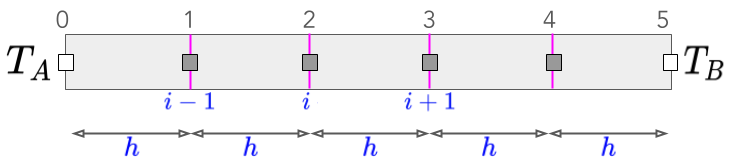
\includegraphics[scale=0.30]{ModCon05.png}$$
	Observe que todas las celdas son de la misma longitud $h$: la malla es 
	\textcolor{blue}{\textit{estructurada}} y \textcolor{blue}{\textit{uniforme}}. 

	\item La aproximación de la derivada se escribe como sigue:
\begin{equation}\label{eq:segundaDer1D}
\boxed{
\left.\frac{d^2 T}{d x^2}\right|_i = \frac{T_{i+1} - 2 T_{i} + T_{i-1}}{h^2} + \mathcal{O}(h^2)
}
\end{equation}
\end{itemize}
}

\end{frame}

\begin{frame}{Discretización de las ecuaciones}

Ahora sustituimos la ecuación \eqref{eq:segundaDer1D} en \eqref{eq:conduccion1D} para obtener:
	\begin{equation}\label{eq:heatDiscreta1D}
	-\kappa_i \left( \frac{T_{i+1} - 2 T_{i} + T_{i-1}}{h^2} \right) = S_i
	\end{equation}
Esta ecuación representa la conducción de calor en el
nodo $i$, y hace uso de sus vecinos $i+1$ e $i-1$.
En este ecuación, tanto $\kappa_i$ como $S_i$ representan la conductividad térmica
y la fuente en el nodo $i$,

\strut

Podemos reescribir la ecuación \eqref{eq:heatDiscreta1D} como sigue:
%
\begin{equation}\label{eq:eqDiscreta1D}
\boxed{-r_i T_{i-1} + 2r_i T_{i} - r_i T_{i+1} = S_i}
\end{equation}
donde $\displaystyle r_i = \frac{\kappa_i}{h^2}$ .

\end{frame}

\begin{frame}{Discretización de las ecuaciones}

En el caso que estamos estudiando, necesitamos calcular la temperatura
en los nodos $i = 1, 2, 3, 4$, que son los nodos internos.
$$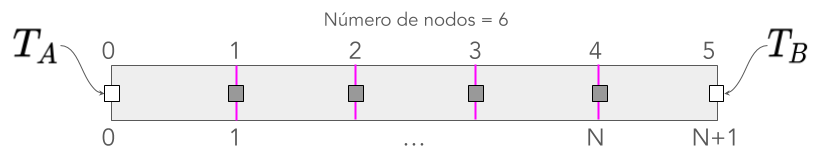
\includegraphics[scale=0.30]{ModCon04.png}$$

Debemos escribir una ecuación para cada uno de esos nodos:
%
\begin{columns}
\begin{column}{0.5\textwidth}
\begin{eqnarray*}
	-r_1 T_{0} + 2r_1 T_{1} - r_1 T_{2} & = & S_1 \\
	-r_2 T_{1} + 2r_2 T_{2} - r_2 T_{3} & = & S_2 \\
	-r_3 T_{2} + 2r_3 T_{3} - r_3 T_{4} & = & S_3 \\
	-r_4 T_{3} + 2r_4 T_{4} - r_4 T_{5} & = & S_4 
\end{eqnarray*}
\end{column}
\begin{column}{0.5\textwidth}
Este es un sistema lineal que debemos resolver para obtener la temperatura en cada
uno de los nodos internos.
\end{column}
\end{columns}

\end{frame}

\begin{frame}{Discretización de las ecuaciones}

Para incorporar las \textbf{condiciones de frontera} debemos modificar las ecuaciones para los nodos en los extremos: $i = 1$ e $i = 4$
%
$$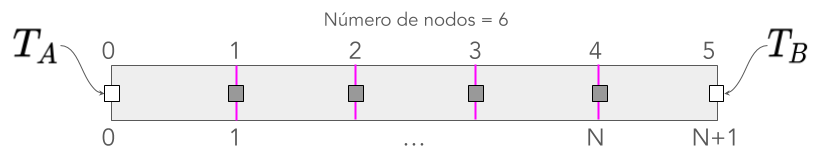
\includegraphics[scale=0.30]{ModCon04.png}$$
%

{\small 
\begin{columns}
\pause
	\begin{column}{0.45\textwidth}
	Para $i=1$ tenemos $T_0  = T_A $
	\begin{eqnarray*}	
	-r_1 T_{0} + 2 r_1 T_{1} - r_1 T_{2} & = & S_1 \\
	-r_1 \boxed{T_{A}} + 2 r_1 T_{1} - r_1 T_{2} & = & S_1
    \end{eqnarray*}
	\[
	\boxed{2 r_1 T_{1} - r_{1} T_{2} = S_1 + r_{1} T_A}
	\]
	\end{column}
\pause
	\begin{column}{0.57\textwidth}
	Para $i = N = 4$ tenemos $T_{N+1} = T_B$
	\begin{eqnarray*}			
	-r_{N} T_{N-1} + 2 r_{N} T_{N} - r_{N} T_{N+1} & = & S_N \\	
	-r_{N} T_{N-1} + 2 r_{N} T_{N} - r_{N} \boxed{T_{B}} & = & S_N 
    \end{eqnarray*}
	\[
	\boxed{-r_{4} T_{3} + 2 r_{4} T_{4} = S_4 + r_{4} T_B}
	\]
	\end{column}
\end{columns}}

Estas dos últimas ecuaciones incorporan las condiciones de frontera de este problema.

\end{frame}

\begin{frame}{Discretización de las ecuaciones}

El sistema de ecuaciones, con las condiciones de frontera
incorporadas, para los nodos $i = 1, 2, 3, 4$, se escribe como sigue:

\begin{eqnarray*}
	2 r_1 T_{1} - r_{1} T_{2} & = & S_1 + r_{1} T_A \\
	-r_2 T_{1} + 2r_2 T_{2} - r_2 T_{3} & = & S_2 \\
	-r_3 T_{2} + 2r_3 T_{3} - r_3 T_{4} & = & S_3 \\
	-r_{4} T_{3} + 2 r_{4} T_{4} & = & S_4 + r_{4} T_B 
\end{eqnarray*}

$$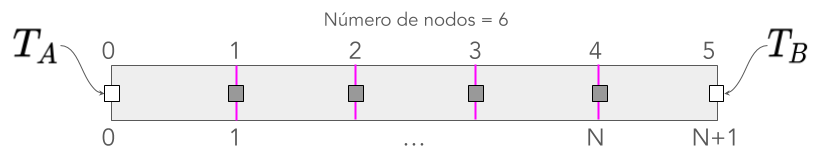
\includegraphics[scale=0.30]{ModCon04.png}$$

\end{frame}


\begin{frame}{Discretización de las ecuaciones}

Podemos ahora escribir, en forma de un sistema lineal, las ecuaciones del problema a resolver,
para cualquier $N$ y para $\kappa = constante$:

\[ 
\underbrace{
	\left[
	\begin{matrix}
	2 & -1 & 0 & 0 & \dots & 0  \\
	-1 & 2 & -1 & 0 & \dots & 0  \\
	0 & -1 & 2 & -1 & \dots & 0  \\
	\vdots & \ddots & \ddots & \ddots & \ddots & \vdots \\
	0 & \dots & 0 & -1 & 2 & -1   \\
	0 & \dots & 0 & 0 & -1 & 2    
	\end{matrix}
	\right]}_{\Tensor{A}_{N \times N}}
\underbrace{
\left[
\begin{matrix}
T_1 \\ T_2 \\ T_3 \\ \vdots \\ T_{N-1} \\ T_N
\end{matrix}
\right]}_{\Vector{T}_N} =
\underbrace{
\frac{1}{r}
\left[
\begin{matrix}
S_1 \\ S_2 \\ S_3 \\ \vdots \\ S_{N-1} \\ S_N
\end{matrix}
\right] +
\left[
\begin{matrix}
T_A \\ 0 \\ 0 \\ \vdots \\ 0 \\ T_B
\end{matrix}
\right]}_{\Vector{b}_N}
\]

donde $\displaystyle r = \frac{\kappa}{h^2}$
\end{frame}

\subsection{Modelo Computacional}

\begin{frame}

{\huge MODELO}
$$
\includegraphics[scale=0.20]{computacionalCOMPLETO}$$

\end{frame}

\begin{frame}{Modelo Computacional}

El objetivo del modelo computacional es escribir programas de cómputo que
permitan obtener las soluciones numéricas del problema descrito en el Modelo Conceptual.
	
{\small
	\begin{itemize}
		\item En este caso se intenta obtener la temperatura $T$ en los nodos interiores de la
		malla.
		
		\item Para ello, se debe encontrar la solución a un sistema del tipo:
		\[\Tensor{A} \cdot \Vector{T} = \Vector{b}\]
		donde $\Tensor{A}$ es una matriz de $N \times N$ y $\Vector{b}$ es un vector de tamaño $N$, ambos con coeficientes conocidos.
		
		\item $\Vector{T}$ es un vector que almacenará la solución en los nodos internos.
	\end{itemize}
}

\strut

Existen varias maneras de realizar esta implementación. A continuación mostraremos una muy sencilla.

\end{frame}

\lstset{language=python,
literate=
	{á}{{\'a}}1
	{Á}{{\'A}}1
	{é}{{\'e}}1
	{É}{{\'E}}1
	{í}{{\'i}}1
	{Í}{{\'I}}1
	{ó}{{\'o}}1
	{Ó}{{\'O}}1
	{ú}{{\'u}}1
	{Ú}{{\'U}}1
	{ñ}{{\~n}}1
}
\lstset{keywordstyle=\color{blue}}
%\lstset{backgroundcolor=\color{classicrose}}
\lstset{basicstyle=\tiny\ttfamily}
\lstset{commentstyle=\color{gray}}
\lstset{frame=trbl}
\lstset{showstringspaces=false}

\begin{frame}[fragile]{Ejemplo 1: Modelo computacional sencillo}

\begin{block}{}

\begin{columns}[t]
\begin{column}{0.48\textwidth}
\begin{lstlisting}
import numpy as np
import matplotlib.pyplot as plt
def buildMatrix(N):
    # Matriz de ceros
    A = np.zeros((N,N))
	
    # Primer renglón
    A[0,0] = 2
    A[0,1] = -1
    # Renglones interiores
    for i in range(1,N-1):
        A[i,i] = 2
        A[i,i+1] = -1
        A[i,i-1] = -1
    # Último renglón
    A[N-1,N-2] = -1
    A[N-1,N-1] = 2
	
    return A

# Parámetros físicos
L = 1.0
TA = 1
TB = 0
k = 1.0
S = 0.0
# Parámetros numéricos
N = 4
h = L / (N+1)
r = k / h**2
\end{lstlisting}		
\end{column}
\begin{column}{0.48\textwidth}
\begin{lstlisting}

# Arreglo para almacenar la solución
T = np.zeros(N+2)
T[0]  = TA  # Frontera izquierda
T[-1] = TB  # Frontera derecha

# Lado derecho del sistema
b = np.zeros(N)
b[:] = S / r # Fuente o sumidero
b[0]  += T[0]   # Condición de frontera
b[-1] += T[-1]  # Condición de frontera

# Construcción de la matriz
A = buildMatrix(N)

# Solución del sistema lineal
T[1:N+1] = np.linalg.solve(A,b)

# Impresión y graficación de la solución
print(T)
x = np.linspace(0, L, N+2)
plt.figure(figsize=(10,7))
plt.plot(x, T, c='grey', lw=2.0)
plt.scatter(x, T, edgecolor='k', zorder= 10)
plt.xlabel('$x$')
plt.ylabel('$T$')
plt.grid()
plt.show()
\end{lstlisting}		
\end{column}
\end{columns}
\end{block}

\end{frame}

\begin{frame}[fragile]{Ejemplo 1: Modelo computacional sencillo}

\begin{block}{Salida del código anterior:}
\begin{verbatim}
T =  [1.  0.8 0.6 0.4 0.2 0. ]
\end{verbatim}
$$ \includegraphics[scale=0.35]{num_cond01}$$
\end{block}
\end{frame}

\section{Ejercicio 2.}

\begin{frame}[fragile]
	
{\small 
\begin{exampleblock}{Ejercicio 2.}
\begin{enumerate}
	\item Abrir la notebook \texttt{E02\_ConduccionEst.ipynb}, del repositorio \href{https://github.com/luiggix/Mixbaal}{\texttt{Mixbaal}}, 
	y escribir el código del ejemplo 1 como sigue:
 	\begin{enumerate}[a]
		\item {\footnotesize Celda 1: La función \texttt{buildMatrix(N)}.}
		\item {\footnotesize Celda 2: Los parámetros físicos y numéricos.}
		\item {\footnotesize Celda 3: El código que resuelve el problema y grafica la solución.}
	\end{enumerate}
	Ejecutar las tres celdas en orden y reproducir la salida del ejemplo 1.
	\item El problema definido en \eqref{eq:conduccion1D} tiene la siguiente solución analítica:
	$$\displaystyle
	T(x) =
	\boxed{\left(\frac{T_B - T_A}{L} + \frac{S}{2\kappa} \left(L - x\right) \right)x + T_A}
	$$
	En la misma notebook del punto 1, agregar 
	\begin{enumerate}[a]
	\item El código para calcular la solución analítica:
	\end{enumerate}
\begin{lstlisting}
def solExact(x, TA, TB, k, L, S):
    """
    Cálculo de la solución exacta.
    """
    return ((TB-TA)/L+(S/(2*k))*(L-x))*x+TA
\end{lstlisting}

\end{enumerate}
\end{exampleblock}
}
\end{frame}


\begin{frame}[fragile]
	
{\small 
\begin{exampleblock}{Ejercicio 2.}

\begin{enumerate}[b]
\item Agregar la siguiente función para el cálculo de la solución numérica:
\begin{lstlisting}
def solNum(L, N, k, S, A, b, T, etiqueta):
    h = L / (N+1)
    r = k / h**2
    
    # Lado derecho del sistema
    b = np.zeros(N)
    b[:] = S / r # Fuente o sumidero
    b[0]  += T[0]   # Condición de frontera
    b[-1] += T[-1]  # Condición de frontera
    
    # Solución del sistema lineal
    T[1:N+1] = np.linalg.solve(A,b)
    
    # Impresión y graficación de la solución
    x = np.linspace(0, L, N+2)
    
    # Construcción de la etiqueta de cada gráfica
    if etiqueta == 'L':
        etiqueta = '$L$ = {:3.2f}'.format(L)
    elif etiqueta == 'k':
        etiqueta = '$\kappa$ = {:3.2f}'.format(k)
    elif etiqueta == 'S':
        etiqueta = '$S$ = {:3.2f}'.format(S)
    
    # Se grafican los puntos de la solución
    plt.scatter(x, T, edgecolor='k', s=50, zorder= 10, label=etiqueta)
\end{lstlisting}

\end{enumerate}
\end{exampleblock}
}
\end{frame}

\begin{frame}[fragile]
	
{\small 
\begin{exampleblock}{Ejercicio 2.}

\begin{enumerate}[c]
\item Agregar la siguiente función para la graficación:

\begin{lstlisting}
def plotSol(title, filename):
    plt.suptitle('Conducción estacionaria',fontsize=24,y=0.94,va='center_baseline')
    plt.title(title, fontsize=20, color='blue')
    plt.ylabel('$T$')
    plt.xlabel('$x$')
    plt.legend(loc='center left', bbox_to_anchor=(1, 0.5), fontsize=12)
    plt.grid()
    plt.savefig(filename)
    plt.show()
\end{lstlisting}
\end{enumerate}
\begin{enumerate}
\setcounter{enumi}{2}
\item Agregar el siguiente código para variar la longitud del dominio ($L$): \label{en:codigo}
\begin{columns}[t]
\begin{column}{0.48\textwidth}
\begin{lstlisting}
# Parámetros físicos
l = [0.25, 0.5, 0.75, 1.0, 1.5, 2.0, 3.0]
TA = 1.0
TB = 0.0
k = 1.0
S = 1.0
# Parámetros numéricos
N = 10

# Arreglo para almacenar la solución
T = np.zeros(N+2)
T[0]  = TA  # Frontera izquierda
T[-1] = TB  # Frontera derecha
\end{lstlisting}		
\end{column}
\begin{column}{0.48\textwidth}
\begin{lstlisting}
# Construcción de la matriz
A = buildMatrix(N)

for L in l:
    solNumerica(L, N, k, S, A, b, T, 'L')
    xe = np.linspace(0,L,100)
    plt.plot(xe, 
             solExacta(xe, TA, TB, k, L, S), 
             'k-', lw=1.0, alpha=0.5)

plotSol('$\kappa$ = {:3.2f}'.format(k) + 
        '$S$ = {:3.2f}'.format(S), 
        'nombre_archivo.pdf')
\end{lstlisting}		
\end{column}
\end{columns}

\end{enumerate}
\end{exampleblock}
}
\end{frame}

\begin{frame}[fragile]
	
{\small 
\begin{exampleblock}{Ejercicio 2.}

Al ejecutar el código anterior deberías obtener algo similar a lo siguiente:
$$\includegraphics[scale=0.30]{L_variable.pdf} $$
Explique el comportamiento de este resultado en términos matemáticos y físicos de la conducción de calor.
\end{exampleblock}
}
\end{frame}

\begin{frame}[fragile]
	
{\small 
\begin{exampleblock}{Ejercicio 2.}
\begin{enumerate}
\setcounter{enumi}{3}
\item Modifica el código del punto \ref{en:codigo} para hacer lo siguiente:
\begin{enumerate}[a]
	\item {\footnotesize $L = 1.0$, $S = 1.0$ y $\kappa = $ \texttt{[0.1, 0.15, 0.25, 0.5, 1.0, 2.0, 10]}.}
	Reproduce la siguiente gráfica:
	$$\includegraphics[scale=0.30]{k_variable.pdf} $$	
\end{enumerate}
\end{enumerate}

\end{exampleblock}
}
\end{frame}

\begin{frame}[fragile]
	
{\small 
\begin{exampleblock}{Ejercicio 2.}
\begin{enumerate}
\setcounter{enumi}{3}
\item cont.
\begin{enumerate}[b]
	\item {\footnotesize $L = 1.0$, $\kappa = 1.0$ y $S = $ \texttt{[-6.0, -4.0, -2.0, 0.0, 2.0, 4.0, 6.0]}.}
	Reproduce la siguiente gráfica:
	$$\includegraphics[scale=0.30]{S_variable.pdf} $$
\end{enumerate}
\end{enumerate}

\end{exampleblock}
}
\end{frame}

\begin{frame}[fragile]
	
{\small 
\begin{exampleblock}{Ejercicio 2.}

\textbf{Nota}: para obtener el mismo estilo de las gráficas de esta presentación, 
deberás usar el siguiente código y ponerlo en una celda al principio del notebook (no olvides ejecutarla).

\begin{lstlisting}
import numpy as np
import matplotlib.pyplot as plt

# Parámetros para el estilo de las gráficas
plt.style.use('seaborn-paper')
params = {'figure.figsize' : (14,7),
          'text.usetex'    : True,
          'xtick.labelsize': 20,
          'ytick.labelsize': 20,
          'axes.labelsize' : 24,
          'axes.titlesize' : 24,
          'legend.fontsize': 24,
          'lines.linewidth': 3,
          'lines.markersize': 10,
          'grid.color'     : 'darkgray',
          'grid.linewidth' : 0.5,
          'grid.linestyle' : '--',
          'font.family': 'DejaVu Serif',
}
plt.rcParams.update(params)
\end{lstlisting}
{\tiny \textcolor{red}{\textbf{OJO}: la línea que contiene el código:} \texttt{'text.usetex' : True} 
 \textcolor{red}{requiere de que tengas instalado \LaTeX en tu computadora. Si no lo tienes, debes comentar esta línea (poner un \texttt{\#} 
 al principio de la línea).}}
\end{exampleblock}
}
\end{frame}

\section<presentation>{Referencias}

\begin{frame}[allowframebreaks]
	%\frametitle<presentation>{Bibliograf\'{\i}a}
	
\begin{thebibliography}{10}
		
{\footnotesize 

% BOOKS 
\beamertemplatebookbibitems

\bibitem{Bergman}
[1] Bergman, T.L. and Incropera, F.P. and DeWitt, D.P. and Lavine, A.S.,
\newblock {\em Fundamentals of Heat and Mass Transfer},
\newblock Wiley, \textbf{2011}.

\bibitem{Leveque}
[2] R.J. Leveque,
\newblock {\em Finite Difference Method for Ordinary and Partial Differential Equations: Steady State and Time-Dependent Problems },
\newblock {Society for Industrial and Applied Mathematics (SIAM), Philadelphia}, \textbf{2007}.

\bibitem{Saad}
[3] Y. Saad
\newblock {\em Iterative Methods for Sparse Linear Systems}.
\newblock PWS/ITP 1996.
\newblock {Online: 
	\textsf{http://www-users.cs.umn.edu/\textasciitilde saad/books.html}, 
	\textbf{2000}}

\bibitem{Burden}
[4]  Richard Burden and J. Douglas Faires
\newblock{\em Numerical Analysis}
\newblock Cengage Learning; 9 edition (August 9, \textbf{2010})

\bibitem{Herrera1} 
[5] I. Herrera \& G. F. Pinder,
\newblock {\em Mathematical Modeling in Science and Engineering: An Axiomatic Approach}, 
\newblock John Wiley \textbf{2012}.

% ARTICULOS    
\beamertemplatearticlebibitems

%\bibitem{Delacruz2011}
%[7]   L. M. de la Cruz,
%\newblock Flujo en una y dos fases en medios porosos: modelos matemáticos, numáricos y computacionales,
%\newblock {\em Reportes técnicos del Instituto de Geofísica}, 2012-4, Agosto \textbf{2012}.


}
		
\end{thebibliography}
\end{frame}

\section{Créditos}

\begin{frame}{Créditos}
	
	\begin{center}
		\textbf{Dr. Luis M. de la Cruz Salas} \\
		\vspace{0.5cm}
		{\small{Departamento de Recursos Naturales}} \\
		\vspace{0.15cm}
		{\small{Instituto de Geof\'isica}} \\ 
		\vspace{0.15cm}
		{\small{Universidad Nacional Aut\'onoma de M\'exico}} \\
		\vspace{0.15cm}
		
\includegraphics[height=.85cm]{unamlogo.png} \\
		\vspace{1.15cm}
		{\scriptsize{Trabajo realizado con el apoyo del Programa UNAM-DGAPA-PAPIME PE101019 \\		
				
\includegraphics[scale=0.20]{ccPyNoxtli.png} }}
	\end{center}
	
\end{frame}

\end{document}
	